\section{Design Decisions and Their Justification}
\label{sec:design}

The proposal fixed the method at the level of Fig.~\ref{fig:pipeline}. Implementing it forced a number of concrete choices. This section records each choice with its reason, and states where it refines or departs from the proposal. The current Look/Check implementation is tested separately from the historical Retell runs. New Retell training is deferred; the retained pathway below describes its architecture, not a newly evaluated correction system.

\begin{figure*}[t]
\centering
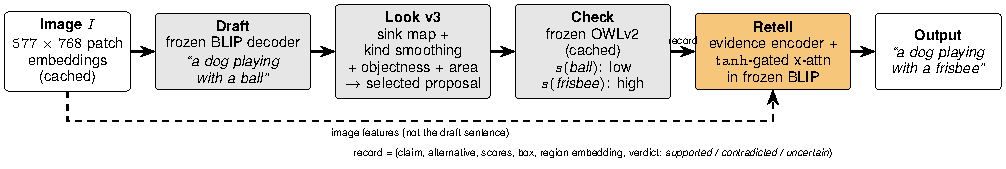
\includegraphics[width=\textwidth]{figures/pipeline.pdf}
\caption{Look--Check--Retell. Grey blocks are frozen; only the evidence encoder and the gated blocks (orange) are trained. Retell receives the image and the verification records, not the draft sentence, so it regenerates the caption; it does not edit it.}
\label{fig:pipeline}
\end{figure*}

\subsection{Frozen Captioner and Shared Visual Features}
\label{sec:design-captioner}
\textbf{Decision.} The drafting model is BLIP-base~\cite{li2022blip}, initialised from the public captioning checkpoint. On Flickr8k we fine-tune only its text decoder and keep the ViT image encoder frozen.

\textbf{Justification.} With a frozen encoder, the $577\times768$ patch embeddings of an image never change. We compute them once, store them in half precision, and every later stage reads them from disk: decoder fine-tuning, drafting, attention extraction, Retell training and all baselines. This has three consequences. (i) Every compared system sees \emph{bit-identical} visual input, which removes one source of uncontrolled variation between B0, B0+, B2, B3 and LCR. (ii) The attention grid that Look relies on keeps a fixed geometry. (iii) Training steps touch only the 12-layer decoder, so every training run in this report takes minutes on a single GPU (we used one Colab A100 for all runs). The proposal spoke of fine-tuning BLIP without saying which parts; freezing the encoder is our reading of it, and we flag it as a choice that trades a small amount of caption quality for control and speed.

\subsection{Held-Out Drafts}
\textbf{Decision.} The 6{,}000 training images are split by a seeded permutation into disjoint halves A and B of 3{,}000 images. The decoder is fine-tuned on A. Its drafts on B train the Retell pathway, and its drafts on validation and test are used for evaluation.

\textbf{Justification.} A captioner drafts images from its own training set unusually well, so the errors it makes there are neither as frequent nor of the same kind as its test-time errors. A pathway trained on such drafts would see evidence that almost always agrees with the claim. With the A/B split, Retell is trained and tested on drafts of images the captioner has not been fine-tuned on. The scripts refuse to draft a half with the decoder that was trained on it.

\subsection{Claim Vocabulary and Extraction}
\label{sec:design-claims}
\textbf{Decision.} $V$ contains \NumClasses{} classes with \NumSurface{} surface forms, curated by hand from the nouns that occur at least 30 times in the training captions. Synonyms share a class (\emph{bicycle}/\emph{bike}, \emph{couch}/\emph{sofa}); all person words form the class \emph{person}. Each class has a \emph{kind}: \emph{person}, \emph{thing} (\NumThing{} countable objects) or \emph{stuff} (\NumStuff{} amorphous regions such as \emph{water}, \emph{grass}, \emph{beach}). A caption word becomes a claim if a part-of-speech tagger marks it as a noun, it maps to a class, and it is not the modifier of a following vocabulary noun (\emph{water bottle} claims a bottle, not water). Each caption contributes at most one claim per class.

\textbf{Justification.} We first tried to build $V$ automatically from WordNet~\cite{miller1995wordnet} categories. The result was unusable: \emph{table} and \emph{forest} are filed under groups, \emph{bikini} under locations. A fixed, human-readable list is also what makes the fairness rule enforceable, since no person word can ever be ``corrected'' into another. We exclude body parts (they belong to a person or animal that is already checked), sport names that are ambiguous with the ball (\emph{football}), and placeholders such as \emph{something}. The \emph{kind} label is an addition to the proposal. A box detector cannot localise \emph{water} or \emph{snow} the way it localises a frisbee, and Section~\ref{sec:exp-check} shows that this distinction matters, so we report the kinds separately throughout.

\subsection{Look: Attention to Region}
\label{sec:design-look}
\textbf{Decision.} After drafting, the finished caption is replayed with teacher forcing. Look reads cross-attention at the position predicting the first word piece of each claim, using the four previously selected E3 heads. The caption-wide mean is subtracted before pooling and rectification, and the map is normalised. The selected heads and person smoothing/SAM rule remain frozen. This is a post-hoc, caption-contrastive map; good localisation does not by itself establish causal dependence of the prediction on that region~\cite{jain2019attention}.

\textbf{Region selection.} For a cached OWLv2 proposal $b$, attention mass and query-independent selection score are
\begin{align}
m_A(b)&=\sum_{i,j}A_{ij}\frac{|c_{ij}\cap b|}{|c_{ij}|},\\
r(b)&=\frac{m_A(b)}{\max(a(b),\epsilon)^{\alpha}}\max(o(b),\epsilon)^{\gamma},
\label{eq:lookv2}
\end{align}
where $a(b)$ is normalised area and $o(b)$ is objectness. For non-person claims, Look retains up to three finite, positive-area proposals with positive attention evidence, ranked by $r$. The old two-patch minimum side filter is removed after its B-only ablation: it excluded tight boxes of visible small objects. The area exponent remains $\alpha=\LookAlpha$; the existing kind-specific objectness exponents remain fixed. No claim-specific detector score enters this ranking. Person claims retain their SAM geometry and explicitly marked nearest-OWL-proposal score proxy.

\textbf{Justification.} Attention supplies the location, while the detector supplies object evidence there. Treating the attention map, the chosen box, and that proposal's classification feature as three separate stages exposes failures that a single end-to-end score hides. The sink correction is our caption-baseline adaptation, motivated by attention sinks~\cite{darcet2024vision}. The head selection, box ranking, and three-candidate aggregation are project choices evaluated on B, rather than claimed reproductions of a cited method.

\textbf{Independent localisation target.} Flickr30k Entities~\cite{plummer2015flickr30k} supplies human-drawn boxes for the Flickr8k images. Reference noun phrases are mapped to our vocabulary and all matching boxes are collected per class. A selected proposal succeeds when its maximum IoU with any matching box reaches the fixed threshold. This measures class-level localisation, rather than exact referent identity; claims without matching annotated boxes are counted but excluded from localisation accuracy. Pointing uses the peak patch centre; energy uses the exact geometric union of the human boxes, counting overlaps once. The boxes are used for evaluation and a small hyperparameter search on B, not model training. Test annotations are not read.

\textbf{Coordinates.} BLIP resizes the image to $384\times384$ without preserving the aspect ratio, so its patch grid is uniform in normalised image coordinates. OWLv2 pads the image to a square at the bottom or right before resizing, so its boxes are relative to a square of side $\max(W,H)$. We convert both to coordinates normalised by the original width and height. Unit tests check the conversion on landscape and portrait images, where a box covering the unpadded area must map exactly to the full image.

\subsection{Check: Cached Open-Vocabulary Verification}
\label{sec:design-check}
\textbf{Decision.} OWLv2 runs once per image. After non-maximum suppression (IoU $0.5$) we keep the 100 proposals with the highest objectness and cache, for each, the box, the objectness, the normalised 512-d class embedding $\mathbf{z}$, and two scalars: the logit shift $\beta$ and scale $\gamma$ that the class head predicts for that proposal. The probability that proposal $p$ shows class $c$ with text embedding $\mathbf{q}_c$ is then
\begin{equation}
s_p(c)=\sigma\!\big(\gamma_p\,(\mathbf{z}_p^{\top}\mathbf{q}_c+\beta_p)\big).
\label{eq:owl}
\end{equation}

\textbf{Justification.} The proposal planned to cache the class embedding only. Reading the detector's class head showed that this is not sufficient: without $\beta_p$ and $\gamma_p$ the scores cannot be reproduced. With them, Eq.~\eqref{eq:owl} gives the detector's exact output for \emph{any} later text query from the cache alone. This is what makes synthetic corruption cheap, since a corrupted label only needs a new dot product. The cache takes about 100\,kB per image.

\textbf{Verification evidence (S4).} The detector is unchanged and frozen; S4 works on its raw logits $\ell_p(c)=\gamma_p(\mathbf{z}_p^{\top}\mathbf{q}_c+\beta_p)$, the argument of Eq.~\eqref{eq:owl}. A wrong object word usually names something that looks like the true object, so the claim is scored against its rivals on the same proposal. Each class $c$ belongs to at most one hand-made set $S(c)$ of mutually exclusive names (for example dog, cat and horse; shirt, jacket and sweater). The rival-aware evidence is
\begin{equation*}
v_p(c)=\ell_p(c)-w\max\!\Big(0,\ \max_{j\in S(c)}\ell_p(j)-\ell_p(c)\Big),\qquad w=\CSRivalWeight,
\end{equation*}
and $v_p(c)=\ell_p(c)$ for a class without rivals. Let $R$ be Look's top-three proposals. The region evidence is $R_c=\max_{p\in R}v_p(c)$ and the image evidence is $X_c=\max_p v_p(c)$ over all proposals. With a per-class threshold $\tau_c$, every non-person claim receives one of five actions:
\begin{equation*}
\text{action}=\begin{cases}
\textit{skip} & \text{no candidate region, no }\tau_c\text{, or a non-visual idiom or compound (``at the camera'', ``hot dog'')},\\
\textit{keep} & R_c\ge\tau_c,\\
\textit{keep\_elsewhere} & R_c<\tau_c\le X_c,\\
\textit{replace} & X_c<\tau_c\text{ and a rival }j\in S(c)\text{ on Look's top-1 box has }\ell(j)\ge\tau_j,\ \ell(j)>\ell(c),\\
\textit{remove} & \text{otherwise.}
\end{cases}
\end{equation*}
\emph{Keep} is a supported verdict, \emph{keep\_elsewhere} and \emph{skip} are uncertain, and \emph{replace} and \emph{remove} are contradicted. Among qualifying rivals, the substitute is the one whose logit lies furthest above its class centre, the median image-level logit of its clean positives shrunk toward its kind. One attended proposal can therefore support a claim, while a contradiction requires that the claim is absent everywhere in the image; detecting the object elsewhere is reported separately rather than counted as support for the attended region. The evidence box stored with a decision is the box whose score made it: the proposal with the largest $v_p(c)$ for a keep, Look's top-1 proposal for a replacement.

\textbf{Calibration and limitations.} Thresholds use only B. Proxy positives for class $c$ are images whose references mention it at least twice, proxy negatives are images whose references never mention it, and $F_p$, $F_u$ are the distributions of $X_c$ in the two groups. Each class gets the cost-sensitive threshold
\begin{equation*}
\tau_c=\arg\max_{\tau}\big[F_u(\tau)-\lambda F_p(\tau)\big]
\end{equation*}
with one $\lambda$ for all classes; classes with fewer than two positives get no threshold and are never contradicted (\CSNoTau{} class). $\lambda=\CSLambda$ is the operating point with the highest out-of-fold false-contradiction rate on reference-supported thing claims that stays at or below \CSTarget\% in five image folds, and the final thresholds are refitted on all of B. These labels are automatic proxies: a reference need not mention every visible object, and a mention does not prove visibility. The components were found by an exploratory review on the same B folds, so the results in Section~\ref{sec:experiments} are a pre-registered reproduction, not an independent estimate. Calibration still counts reference mentions in the non-visual idioms that the live check skips; correcting this moves a few thresholds and is pending. No language prior, captioner-consistency signal, VQA or second verifier enters Check.

\subsection{Retell: Gated Evidence Pathway}
\label{sec:design-retell}
\textbf{Retained architecture; new training deferred.} An evidence encoder maps each inspected region to one 768-d token,
\begin{equation*}
\mathbf{t}=\mathrm{LN}\big(W_c\,\mathbf{w}_c+W_a\,\mathbf{w}_a+f([\mathbf{z}_r;\mathbf{g}])+\mathbf{v}_{\text{verdict}}\big),
\end{equation*}
where $\mathbf{w}_c,\mathbf{w}_a$ are BLIP's own frozen word embeddings of the claimed and alternative labels, $f$ is a two-layer MLP over the region embedding and nine scalars $\mathbf{g}$ (scores, excess mass, box geometry, a has-region flag), and $\mathbf{v}$ is a learned verdict embedding. A learned \emph{null token} is always prepended. Before each of the upper six decoder layers we insert a gated block in the style of Flamingo~\cite{alayrac2022flamingo}:
\begin{align}
\mathbf{h}&\leftarrow\mathbf{h}+\tanh(\alpha_1)\,\mathrm{XAttn}\big(\mathrm{LN}(\mathbf{h}),T\big),\\
\mathbf{h}&\leftarrow\mathbf{h}+\tanh(\alpha_2)\,\mathrm{FF}\big(\mathrm{LN}(\mathbf{h})\big),
\end{align}
with $T$ the evidence tokens and $\alpha_1=\alpha_2=0$ at initialisation. The frozen BLIP layer then runs unchanged. The pathway has \ParamsM{}\,M trainable parameters; BLIP and OWLv2 are frozen.

\textbf{Justification.} \emph{Zero-initialised gates.} Since $\tanh(0)=0$, the system starts as the frozen captioner exactly, which we verify in Section~\ref{sec:exp-gate}. Training can only move away from B0 if doing so lowers the captioning loss, and the learned gate values show directly how much each layer uses the pathway. \emph{Labels in BLIP's own embedding space.} The decoder already knows how to turn its word embeddings into output words, so expressing ``the alternative is \emph{frisbee}'' in that space makes the useful behaviour easy to learn from little data. \emph{Null token.} With it, cross-attention is defined when an image has no records, and the no-evidence control B0+ can use the identical architecture. \emph{Upper layers only.} Object identity is decided late in the decoder; restricting the pathway to six layers halves its size, which matters with only 3{,}000 training images. \emph{Regeneration.} Retell is not given the draft sentence. Draft information enters only through the records, so swapping a record and observing the output is a clean test of whether evidence is used.

\textbf{Training.} The target is one of the five reference captions with the standard captioning loss. Each record is dropped with probability $0.15$ so that the model also learns to caption without it.

\subsection{Synthetic Claim Corruption}
\textbf{Decision.} With probability $\rho$, a non-person training claim has its label replaced by a wrong one, the scores and verdict are recomputed for the same region with Eq.~\eqref{eq:owl}, and the original label joins the alternatives. As the wrong label we first take the captioner's own next-best vocabulary word at that position, provided no reference mentions it; if there is none, we fall back to a class with a similar co-occurrence context in the training captions.

\textbf{Justification.} Natural draft errors are rare, so most training records simply confirm the draft. Corruption creates records in which claim and visual evidence disagree, following LURE~\cite{zhou2024analyzing}. The proposal specified a frequently co-occurring noun. We prefer the captioner's runner-up word because hallucinations follow the language prior~\cite{rohrbach2018object}, and the runner-up is by construction the error this particular captioner was closest to making. No label tells the model to trust the evidence; the only supervision is still the reference captions.

\subsection{Matched Controls}
All trained systems share the frozen captioner, the pathway architecture, the optimiser and the number of updates, and differ only in the tokens they receive: LCR receives records for attention-selected regions; \textbf{B3} receives records for the region with the highest detector score for the claim; \textbf{B2} receives up to six image-level detector tags; \textbf{B0+} receives only the null token. B0+ is the control that matters most. Retell training shows the pathway 3{,}000 images that the captioner has not been fine-tuned on, so a caption can improve merely because of that extra data. Any claim about evidence must therefore be made relative to B0+, not to the draft B0.

\subsection{Evaluation Design}
\label{sec:design-eval}
\textbf{Paired analysis of the primary hypothesis.} H1 asks for a 15\% relative reduction of the human-verified incorrect claim rate (HICR). We computed how many claims this needs. Treating the two systems as independent samples, a two-proportion test at $\alpha=0.05$ and 80\% power needs the numbers in Table~\ref{tab:power} (left); at a draft error rate of 8\% that is \HPowerIndepEight{} claims per system, far beyond 400 annotated images. But the two systems caption the \emph{same} images and most claims are identical in both outputs. Only the claims that change carry information, which is the setting of an exact paired sign test~\cite{koehn2004statistical}. Table~\ref{tab:power} (right) simulates its power at exactly H1's effect: with 1\% of correct claims broken, a 15\% reduction at a draft error rate of 8\% requires fixing \HPowerFixEight{} of the draft errors, and then 1{,}000 traced draft claims give \HPowerEightOneK\% power and 2{,}000 give \HPowerEightTwoK\%; at 5\%, 2{,}000 claims give \HPowerFiveTwoK\% and 4{,}000 give \HPowerFiveFourK\%. These figures are optimistic in two ways. Claims of the same image are treated as independent, although they share an image and a caption, so the effective sample is smaller. And the sign test traces draft claims only, whereas HICR also counts objects that Retell adds; a system can repair draft claims and still raise HICR, so both are reported. The pilot error rate therefore decides whether H1 is testable at all. \emph{Decision:} H1 will be tested on paired, claim-traced outcomes with image-level bootstrap intervals. The final $N$ will be fixed from the pilot error rate before any system is run on test.

\textbf{Annotation tool.} We built an offline annotation page that shows each unique (image, caption) pair once, hides the system identity, shuffles items so that versions of one image are not adjacent, and asks for a label for every object noun, including nouns outside $V$. A scoring script computes HICR, fix, break and net repair rates, Cohen's $\kappa$~\cite{cohen1960coefficient} and bootstrap intervals from the exported files.

\textbf{Reproducibility.} Every number in Sections~\ref{sec:design} and~\ref{sec:experiments} is written into this document by the script that computed it; none is typed by hand.

\begin{table}[t]
\caption{Sample size for H1 (15\% relative HICR reduction, $\alpha=0.05$). Left: claims per system for an
independent two-proportion test at 80\% power. Right: simulated power of the paired sign test with $N$ traced
draft claims at exactly that effect: 1\% of correct claims are broken and the fix rate is set so that HICR falls
by 15\%. Optimistic: claims of one image are treated as independent, and objects added by Retell are not traced.}
\label{tab:power}
\centering\footnotesize
\begin{tabular}{@{}crc|cccc@{}}
\toprule
Draft error & Independent & Fix & \multicolumn{4}{c}{Paired power at $N$ claims} \\
rate $p_0$ & claims needed & rate & 500 & 1{,}000 & 2{,}000 & 4{,}000 \\
\midrule
5\% & 12{,}309 & 0.34 & 12\% & 23\% & 50\% & 82\% \\
8\% & 7{,}469 & 0.27 & 24\% & 52\% & 85\% & 99\% \\
12\% & 4{,}780 & 0.22 & 49\% & 83\% & 99\% & 100\% \\
\bottomrule
\end{tabular}
\end{table}

